Our approach was inspired by Steder \textit{et al.} \cite{steder2008visual}, who  presented a system that allows aerial vehicles to acquire visual maps of large environments using comparable setup with an inertial sensor and a low-quality camera pointing downward. In their approach the inertial sensor was used to estimate a number of parameters in the spatial relation between two camera poses, which reduces the dimensionality of the pose to be estimated.
Equivalent with our approach, Steder uses Speeded-Up Robust Features (SURF) \cite{Bay2008cviu} that are invariant with respect to rotation and scale.
By matching features between different images, one can estimate the relative motion of the camera and construct the graph that serves as input to the TORO-based network optimizer \cite{Grisetti2007iros}.
%SLAM algorithm \cite{Grisetti2007iros}.
%In contrast to our approach, the attitude sensor provides not only the attitude, but also the roll and pitch angle of the camera. This valuable information could be directly integrated into the estimate.

%\begin{comment}
While Steder uses a Euclidean distance measure to compare the correspondences of the features in two images, Caballero \textit{et al.} \cite{caballero2009unmanned} indicate that this is a last resort. They are able to make a robust estimation of the spatial relationship on different levels: homogeneous, affine and Euclidean. First an attempt is made to estimate complete homogeneous transformation (8 degrees of freedom). When the number of correspondences is too low an affine transformation (6 degrees of freedom) is estimated. Only when the features in the image are really noisy a Euclidean transformation (4 degrees of freedom) is estimated.
%\end{comment}

Since the 2011 summer edition of the Micro Air Vehicle competition, a team can choose to either use a standard platform or create their own.
Prior to 2011 no standard platform existed in the competition, resulting in participants to focus on constructing optimal sensor configurations.
%in the Micro Air Vehicle competition\footnote{\url{http://www.emav2009.org}, \url{http://www.imav2010.org}}.
%which allowed to participants to construct optimal sensor configurations.
For instance, \cite{Bachrach2009ijmav} describes a quadrotor equipped a Hokuyo laser scanner, allowing many techniques developed for ground robotics to be applied on their flying robot.
Another example is the approach from \cite{Stowers2009ijmav}, where an omnidirectional camera was mounted on the platform, which was used to acquire a heading estimation from the optical flow.
% of the team from Canterbury
At the %latest edition of the Micro Air Vehicle competition
Spring 2011 Micro Air Vehicle competition\footnote{\url{http://www.springimav2011.com}} a Parrot AR.Drone was extended with an infrared camera to be able to follow people \cite{Jonanov2011}. Because the AR.Drone is a quite recent development, the number of studies based on this platform is limited. A recent publication is from Cornell University \cite{Bills2011icra}, where an AR.Drone is used to automatically navigate corridors and staircases based on visual clues.

\begin{figure}[htb]
\centering
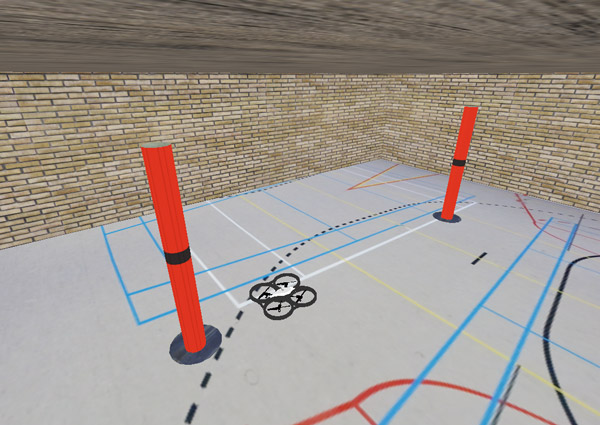
\includegraphics[width=7cm]{images/AR-DroneInGym.jpg}
\caption{3D model of a gym with realistic ground and wall textures which represents the circumstances during the Micro Air Vehicle pylon challenge.}
\label{fig:AR.DroneInGym}
\end{figure}

The other teams during the 2011 summer edition of the IMAV indoor competition relied on detecting the brightly coloured pylons to navigate their drones. In the 2010 edition the PixHawk team \cite{Meier2011} already demonstrated that autonomous navigation is possible by making a visual map from the ground, although they needed artificial texture on the ground. In the method described in this article the natural texture of the ground in the gym is used.

As indicated in \cite{Michael2010ra}, an accurate simulation of a quadrotor is a valuable asset, which allows safe and efficient development of control algorithms. Additionally, it gives direct access to ground truth values and allows to design repeatable experiments.
% STRANGE SENTENCE?
%To be used in such a way, not only the models of the sensors and actuators have to be validated.
Validation of the sensor and actuator models is essential to guarantee 
the utility of both development and experimentation. 
Another useful feature is that the simulation environment is equipped with an editor, which allows detailed modifications to the simulated environment. The details needed for the experiment can be easily added as illustrated in Figure~\ref{fig:AR.DroneInGym}.
%The environment selected is USARSim \cite{Balakirsky2009iros}, which allows physical realistic simulations and a versatile environment editor.


	\section{Simultaneous localization and mapping}
		\subsection{Visual simultaneous localization and mapping}
	\section{International Micro Air Vehicle Competition}
	\section{AR.Drone}